\documentclass[a4paper,12pt]{article}
\usepackage{epsfig,latexsym,amsmath,amssymb,epic,eepic,psfrag,subfigure,float,euscript,array}
\usepackage[latin1]{inputenc}
\usepackage{standalone}
\usepackage{tikz,pgf,pgfplots}

\newenvironment{exercise}[1][Uppgift]{\begin{trivlist} \item[\hskip
    \labelsep {\stepcounter{exerctr}\bfseries #1
      \arabic{exerctr}}]}{\end{trivlist}\vspace{10mm}}

\newcounter{exerctr}
\newcounter{abcctr}[exerctr]

\newcommand{\abc}{\noindent\vspace{1mm}\\ {\bf
    \stepcounter{abcctr}(\alph{abcctr})\ }}
\newcommand{\bbm}{\begin{bmatrix}}
\newcommand{\ebm}{\end{bmatrix}}
\newcommand{\point}[1]{\hfill {\bf (#1p)}\\ \vspace{-5mm}}
\newcommand{\ctrb}{\EuScript{S}}
\newcommand{\Lap}{\mathcal{L}}
\newcommand{\obsv}{\EuScript{O}}
\newcommand{\realdel}[1]{\text{Re}\left\{#1\right\}}
\newcommand{\imagdel}{\text{Im}}
\newcommand{\bC}{\mathbb{C}}
\newcommand{\bR}{\mathbb{R}}
\newcommand{\bmpv}{\begin{minipage}[t]}
\newcommand{\bmps}{\begin{minipage}[t]{45mm}}
\newcommand{\bmpm}{\begin{minipage}[t]{90mm}}
\newcommand{\bmpl}{\begin{minipage}[t]{140mm}}
\newcommand{\emp}{\end{minipage}}
\newcommand*{\zethree}{\big(z - \mexp{-3h}\big)}
\newcommand*{\mexp}[1]{\ensuremath{\mathrm{e}^{#1}}}

\addtolength{\topmargin}{-1cm}
\textheight 23.5cm
%\oddsidemargin 0.61cm
%\evensidemargin 0.61cm


\def\OctaveG{tf([0.5 1], [1 0 -1])}

\title{Computerized control partial exam 1 -- Dummy exam from fall semester 2016}
\author{Kjartan Halvorsen}

\begin{document}

\maketitle


\begin{description}
\item[Time] Whenever suits you best. Each problem should not take more than 30 min to solve. \textbf{The actual exam will have only three problems.}
\item[Place] Somewhere quiet
\item[Permitted aids] For the exam: The single colored page with your own notes, table of Laplace transforms, calculator
\end{description}

All answers should be readable and well motivated (if nothing else is written). Solutions/motivations should be written on the provided spaces in this exam. Use the last page if more space is needed.

\begin{center}
{\Large Good luck!} \\
\end{center}

\begin{tabular}{|l|l|}
\hline
\multicolumn{2}{|l|}{\bmpl
Matricula and name
\vspace*{14mm}
\emp}\\
\hline

\end{tabular}

\clearpage

%-----------------------------------------------------------------
\subsection*{Problem 1}
Consider the continuous-time system with the following transfer function
\[ G(s) = \frac{s+1}{s(s+3)}. \]
The system is sampled with sampling interval $h$ using step-invariant (zero-order hold) sampling. \textbf{Show that the pulse-transfer function for the sampled system is}
\[ H(z) = \frac{(2z-2+3h)\zethree{} - 2(z-1)^2}{9(z-1)\zethree{}}. \]

\noindent
\fbox{
\bmpl
{\bf Derivation:}\\
\vspace*{130mm}
\emp}

\clearpage
\subsection*{Problem 2}

The sampled system in Problem 1 is controlled using proportional control with gain equal to 1. 
\begin{center}
  \includestandalone[width=0.5\linewidth]{feedback}
\end{center}

Calculate the closed-loop pulse-transfer function


\noindent
\fbox{
\bmpl
{\bf Solutions:}\\
\vspace*{130mm}
\emp}

\clearpage
\subsection*{Problem 3}
What is the steady-state value of the control error $e(kh) = y_{ref}(kh) - y(kh)$? when $y_{ref}(kh)$ is a step?

\noindent
\fbox{
\bmpl
{\bf Solution:}\\
\vspace*{70mm}
\emp}

\subsection*{Problem 4 NOT RELEVANT FOR 2017ENE-MAY}
Instead of designing a discrete-time controller, a continuous-time controller was designed, given by
\[ 2\frac{d}{dt} u + u = 2\frac{d}{dt}e + 5e  \]
Discretize the controller using Tustin's approximation. Determine the poles and zeroes of the discrete-time controller.

\noindent
\fbox{
\bmpl
{\bf Solution:}\\
\vspace*{70mm}
\emp}

\clearpage

\subsection*{Problem 5}
Below is a plot of a discrete-time signal $x(k)=\realdel{a^k}$. Mark out $a$ in the complex plane below. Motivate your answer.
\begin{center}
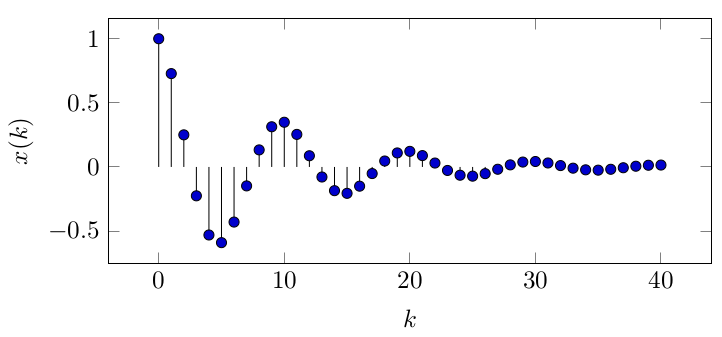
\includegraphics[width=1.0\linewidth]{discrete-signal-decaying-sinusoid.png}
\end{center}

\fbox{
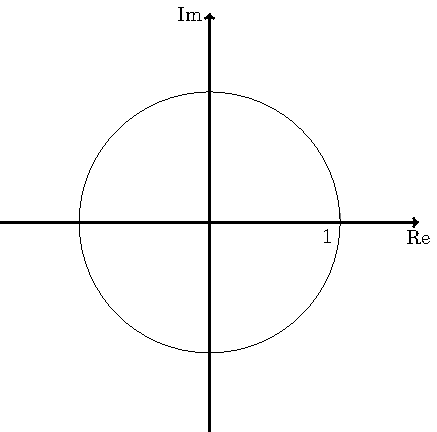
\includegraphics[width=0.4\linewidth]{imaginary-plane-empty}
\bmpm
{\bf Motivation:}\\
\vspace*{70mm}
\emp}

\clearpage

\noindent
{\bf If necessary,} you can continue your solutions on this page. Mark clearly which problem the solution corresponds to.


%\end{document}
%*****************************************************************
%*****************************************************************
\newpage
\setcounter{page}{1}

\section*{Solutions}
\subsection*{Problem 1}
   First calculate the step-response of the continous-time system
   \[G(s)\frac{1}{s} = \frac{s+1}{s^2(s+3)} = \frac{2}{9s} + \frac{1}{3s^2} - \frac{2}{9(s+3)}.\]
   The inverse Laplace-transform gives
   \[ y(t) = \frac{2}{9} + \frac{1}{3}t - \frac{2}{9}\mexp{-3t}. \]
   Sampling this function gives
   \[ y(kh) = \frac{2}{9} + \frac{1}{3}kh - \frac{2}{9}\big(\mexp{-3h}\big)^k, \]
   which has the Z-transform
   \[Y(z) = \frac{2z}{9(z-1)} + \frac{hz}{3(z-1)^2} - \frac{2z}{9\zethree{}}. \]
   Dividing the z-transform of the system response to that of the input (the step) gives
   \begin{align*}
   H(z) &= \frac{Y(z)}{U(z)} = \frac{z-1}{z}Y(z) = \frac{2}{9} + \frac{h}{3(z-1)} - \frac{2(z-1)}{9\zethree{}}\\
        &= \frac{2(z-1)\zethree{} + 3h\zethree{} - 2(z-1)^2}{9(z-1)\zethree{}}\\
	&= \frac{(2z-2+3h)\zethree - 2(z-1)^2}{9(z-1)\zethree{}}.
   \end{align*}


\subsection*{Problem 2}
Write the open-loop pulse-transfer function 
\[ H(z) = \frac{B(z)}{A(z)} = \frac{(2z-2+3h)\zethree - 2(z-1)^2}{9(z-1)\zethree{}}. \]
The closed-loop pulse transfer function from the reference signal to the output becomes
\begin{equation*}
\begin{split}
  H_c(z) &= \frac{H(z)}{1+H(z)} = \frac{B(z)}{A(z) + B(z)}\\
  &= \frac{(2z-2+3h)\zethree - 2(z-1)^2}{ 9(z-1)\zethree{} + (2z-2+3h)\zethree - 2(z-1)^2}
\end{split}
\end{equation*}

\subsection*{Problem 3}
The steady-state control error becomes
\[ \lim_{k\to\infty} \big(y_{ref}(kh) - y(kh)\big) = \lim_{k\to\infty} y_{ref}(kh) - \lim_{k\to\infty}  y(kh). \]
The first limit is simply the steady-state value of the unit step input signal which is $1$. The second limit can be computed using the final value theorem
\begin{equation*}
\begin{split}
  \lim_{k\to\infty} y(kh) &= \lim_{z\to 1} (z-1)Y(z) = \lim_{z\to 1} (z-1)\frac{H(z)}{1+H(z)} Y_{ref}(z)\\
  &= \lim_{z\to 1} (z-1) \frac{B(z)}{A(z) + B(z)} \frac{z}{z-1} = \lim_{z\to 1} \frac{zB(z)}{A(z) + B(z)}\\
  &= \lim_{z\to 1} z \frac{(2z-2+3h)\zethree - 2(z-1)^2}{ 9(z-1)\zethree{} + (2z-2+3h)\zethree - 2(z-1)^2}
  = \frac{3h(1-\mexp{-3h})}{3h(1-\mexp{-3h})} = 1.
\end{split}
\end{equation*}
So the steady-state error is zero. 

\subsection*{Problem 4}
The controller has transfer function

\[ F(s) = \frac{2s + 5}{2s + 1}. \]
Inserting for the Tustin's approximation gives
\begin{equation*}
\begin{split}
  F_d(z) &= F(s)|_{s=\frac{2}{h}\frac{z-1}{z+1}}\\
  &= \frac{2\frac{2}{h}\frac{z-1}{z+1} + 5}{2\frac{2}{h}\frac{z-1}{z+1} + 1}\\
  &= \frac{4(z-1) + 5h(z+1)}{4(z-1) + h(z+1)} = \frac{(4 + 5h)z - (4 -5h)}{(4+h)z - (4 - h)}
\end{split}
\end{equation*}
The pole is in \(z = \frac{4-h}{4+h}\) and the zero in \(z = \frac{4-5h}{4+5h}\).


\subsection*{Problem 5}
$\mathrm{Re}\{a^k\}$ is the operation of taking the real part of the expression $a^k$, where $a$ is a complex number. Seen in the complex plane, we project the point $a^k$ onto the real line in order to find the real part. 

In polar form we have
\[ x(k) = \realdel{\Big(r\mexp{i\theta}\Big)^k}. \]

The discrete-time signal in the graph is a decaying discrete cosine. The period is clearly 10 samples, so we must have
\[ x(k) = \realdel{\Big(r\mexp{i\frac{\pi}{5}}\Big)^k}. \]
The signal is decaying at a rate such that the amplitude is approximately 0.1 after 20 samples.
\[ r^{20} \approx 0.1\]
Hence \[ r \approx 0.1^{1/20} = 0.89 \] (In fact, $r=0.9$)

\end{document} 
